% Research-mode method overview.
% Five-second message: RLB exposes detached local summaries to MatrixPolicy;
% MatrixPolicy uses them to update only the adjacent matrix pair (A_l,B_l).
% Grammar: three horizontal layers--forward map, read-only summaries, policy.
% The caption carries explanatory prose; the diagram keeps labels concise.
\documentclass[11pt,tikz,border=5pt]{standalone}
\usepackage{tikz}
\usepackage{amsmath,amssymb}
\usepackage[T1]{fontenc}
\usepackage{times}
\usetikzlibrary{arrows.meta,calc,positioning}

\definecolor{mpInk}{HTML}{25282D}
\definecolor{mpMuted}{HTML}{687079}
\definecolor{mpLine}{HTML}{A7ADB4}
\definecolor{mpBlue}{HTML}{2F6FA3}
\definecolor{mpBlueFill}{HTML}{EDF4FA}
\definecolor{mpGreen}{HTML}{2B8560}
\definecolor{mpAmber}{HTML}{A86E00}
\definecolor{mpAmberFill}{HTML}{FFF3D2}
\definecolor{mpPurple}{HTML}{6846A3}
\definecolor{mpPurpleFill}{HTML}{F2EDF8}
\definecolor{mpPanel}{HTML}{F7F8F9}

\tikzset{
  every node/.style={font=\small, text=mpInk},
  matrixCard/.style={rectangle, rounded corners=4pt, draw=mpBlue,
    fill=mpBlueFill, line width=0.95pt, minimum width=1.68cm,
    minimum height=1.18cm, inner sep=0pt},
  rlbCard/.style={rectangle, rounded corners=5pt, draw=mpAmber,
    fill=mpAmberFill, line width=1.00pt, minimum width=4.24cm,
    minimum height=1.50cm, align=center, inner sep=5pt},
  summaryBus/.style={rectangle, rounded corners=4pt, draw=mpLine,
    fill=mpPanel, line width=0.68pt, minimum width=9.40cm,
    minimum height=1.16cm},
  policy/.style={rectangle, rounded corners=5pt, draw=mpPurple,
    fill=mpPurpleFill, line width=1.05pt, minimum width=6.04cm,
    minimum height=0.94cm, align=center, inner sep=4pt},
  updateTag/.style={rectangle, rounded corners=3pt, draw=mpPurple!76,
    fill=white, line width=0.72pt, minimum width=1.56cm,
    minimum height=0.48cm, align=center, text=mpPurple,
    font=\footnotesize},
  forward/.style={-{Stealth[length=4.8pt,width=5.2pt]}, line width=0.92pt,
    color=mpInk, shorten >=2pt, shorten <=2pt},
  read/.style={-{Stealth[length=3.4pt,width=3.8pt]}, densely dashed,
    line width=0.58pt, color=mpLine!95, shorten >=1.5pt, shorten <=1pt},
  write/.style={-{Stealth[length=4.4pt,width=4.8pt]}, line width=0.82pt,
    color=mpPurple!88, shorten >=1.5pt, shorten <=1pt},
  fine/.style={font=\footnotesize, text=mpMuted, align=center},
}

\newcommand{\matrixcells}[2]{%
  \foreach \i in {0,...,3} {
    \foreach \j in {0,...,2} {
      \pgfmathsetmacro{\shade}{28+7*\i+7*\j}
      \fill[mpBlue!\shade!white, draw=white, line width=0.28pt]
        ($(#1.center)+(-0.55+0.34*\i,-0.35+0.30*\j)$)
        rectangle ++(0.27,0.22);
    }
  }
  \node[font=\footnotesize\bfseries, text=mpBlue, fill=white,
    inner xsep=2pt, inner ysep=0.5pt] at ([yshift=0.70cm]#1.center) {#2};
}

\begin{document}
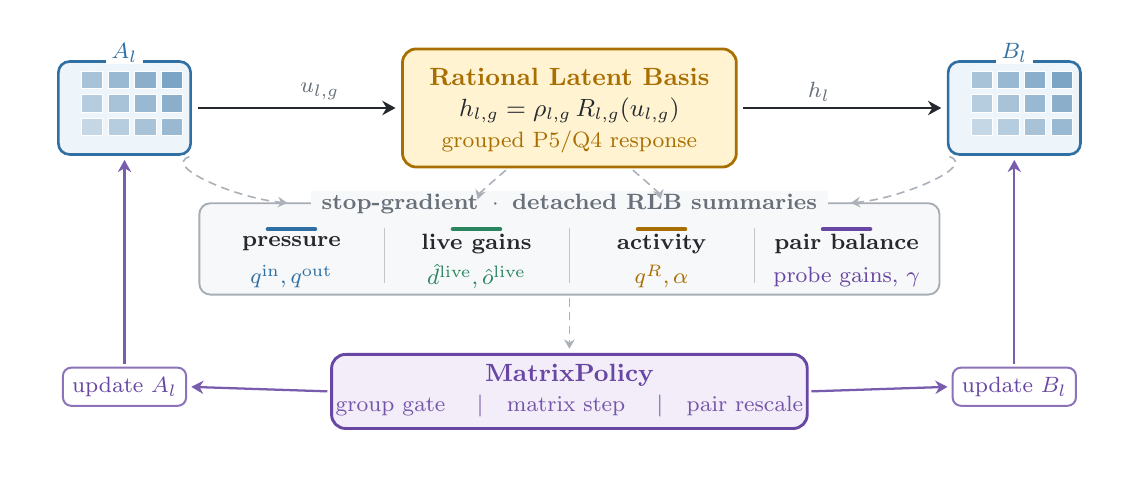
\begin{tikzpicture}[x=1cm,y=1cm]
  \useasboundingbox (0.12,0.18) rectangle (13.88,5.72);

  % Forward activation map.
  \node[matrixCard] (amat) at (1.35,4.70) {};
  \matrixcells{amat}{$A_l$}
  \node[rlbCard] (rlb) at (7.00,4.70) {};
  \node[font=\small\bfseries, text=mpAmber] at ([yshift=0.40cm]rlb.center)
    {Rational Latent Basis};
  \node[font=\small] at ([yshift=-0.03cm]rlb.center)
    {$h_{l,g}=\rho_{l,g}\,R_{l,g}(u_{l,g})$};
  \node[font=\footnotesize, text=mpAmber] at ([yshift=-0.43cm]rlb.center)
    {grouped P5/Q4 response};
  \node[matrixCard] (bmat) at (12.65,4.70) {};
  \matrixcells{bmat}{$B_l$}

  \draw[forward] (amat.east) -- (rlb.west);
  \node[fine, fill=white, inner sep=1.5pt] at (3.83,4.91) {$u_{l,g}$};
  \draw[forward] (rlb.east) -- (bmat.west);
  \node[fine, fill=white, inner sep=1.5pt] at (10.17,4.91) {$h_l$};

  % A single quiet bus replaces four competing cards.
  \node[summaryBus] (bus) at (7.00,2.91) {};
  \node[font=\footnotesize\bfseries, text=mpMuted, fill=mpPanel,
    inner xsep=4pt, inner ysep=1pt] at ([yshift=-0.02cm]bus.north)
    {stop-gradient \,$\cdot$\, detached RLB summaries};
  \foreach \x in {4.65,7.00,9.35} {
    \draw[mpLine!70, line width=0.42pt] (\x,2.48) -- (\x,3.18);
  }

  \draw[mpBlue, line width=1.55pt, line cap=round] (3.17,3.16) -- (3.77,3.16);
  \node[font=\footnotesize\bfseries, text=mpInk] at (3.47,2.97) {pressure};
  \node[font=\footnotesize, text=mpBlue] at (3.47,2.56)
    {$q^{\rm in},q^{\rm out}$};

  \draw[mpGreen, line width=1.55pt, line cap=round] (5.52,3.16) -- (6.12,3.16);
  \node[font=\footnotesize\bfseries, text=mpInk] at (5.82,2.97) {live gains};
  \node[font=\footnotesize, text=mpGreen] at (5.82,2.56)
    {$\hat d^{\rm live},\hat o^{\rm live}$};

  \draw[mpAmber, line width=1.55pt, line cap=round] (7.87,3.16) -- (8.47,3.16);
  \node[font=\footnotesize\bfseries, text=mpInk] at (8.17,2.97) {activity};
  \node[font=\footnotesize, text=mpAmber] at (8.17,2.56)
    {$q^R,\alpha$};

  \draw[mpPurple, line width=1.55pt, line cap=round] (10.22,3.16) -- (10.82,3.16);
  \node[font=\footnotesize\bfseries, text=mpInk] at (10.52,2.97) {pair balance};
  \node[font=\footnotesize, text=mpPurple] at (10.52,2.56)
    {probe gains, $\gamma$};

  \draw[read] (amat.south east)
    .. controls (1.82,3.96) and (2.78,3.55) .. (3.47,3.49);
  \draw[read] ([xshift=-0.78cm]rlb.south)
    .. controls (6.04,3.78) and (5.86,3.62) .. (5.82,3.49);
  \draw[read] ([xshift=0.78cm]rlb.south)
    .. controls (7.96,3.78) and (8.14,3.62) .. (8.17,3.49);
  \draw[read] (bmat.south west)
    .. controls (12.18,3.96) and (11.22,3.55) .. (10.52,3.49);

  % MatrixPolicy is the only emphasized controller.
  \node[policy] (policy) at (7.00,1.10) {};
  \node[font=\small\bfseries, text=mpPurple] at (7.00,1.30) {MatrixPolicy};
  \node[font=\footnotesize, text=mpPurple!92] at (7.00,0.91)
    {group gate \quad$\vert$\quad matrix step \quad$\vert$\quad pair rescale};
  \draw[read] (bus.south) -- (policy.north);

  \node[updateTag] (ua) at (1.35,1.16) {update $A_l$};
  \node[updateTag] (ub) at (12.65,1.16) {update $B_l$};
  \draw[write] (policy.west) -- (ua.east);
  \draw[write] (policy.east) -- (ub.west);
  \draw[write] (ua.north) -- (amat.south);
  \draw[write] (ub.north) -- (bmat.south);
\end{tikzpicture}
\end{document}
